% ju 12-5-22 01-N-Keywords-Thema.tex
\documentclass[a4paper,12pt,fleqn,parskip=half]{scrartcl}
\usepackage[ngerman]{babel}
\usepackage[utf8]{inputenc}
\usepackage[T1]{fontenc}

% Schrift
%\usepackage{lmodern}
\usepackage[osf,sc]{mathpazo} 
\usepackage[scale=.9,semibold]{sourcecodepro}   
\usepackage[osf]{sourcesanspro}  

\usepackage[headsepline]{scrlayer-scrpage}
\pagestyle{scrheadings}
\clearpairofpagestyles

\usepackage[table,dvipsnames,usenames]{xcolor}
\usepackage{textcase}
\usepackage{nameref}
\usepackage{hyperref}
\usepackage{tabularx}
\usepackage{multirow}
\usepackage{multicol}
\usepackage{caption, booktabs}
\usepackage{graphicx} 
\usepackage{scrhack}    
\usepackage{url}%% Links
\usepackage[inline]{enumitem}
\usepackage{pifont}
\usepackage{eurosym}% \euro 20,-
\usepackage{amsmath}
\usepackage{amsfonts}
\usepackage{amssymb}
\usepackage{array}            % Extending the array and tabular environments
\usepackage{chngcntr}         % Change the resetting of counters
\usepackage[version=4]{mhchem}
\usepackage{stmaryrd}
\usepackage{siunitx}
\usepackage{float}
\usepackage{csquotes}
\usepackage{subcaption}
\usepackage{mathtools}
\usepackage{icomma}%Dezimaltrennzeichen
\usepackage{multimedia}%Video: \movie[externalviewer]{(video.mov)}{video.mov}
\usepackage{epstopdf}
\usepackage{footnote}
\usepackage{qrcode}% Anwendung: \qrcode[hyperlink,level=Q,version=2,height=1cm]{\website}
\usepackage{underscore}% Unterstrich ____

% PDF Dokumente einbinden
\usepackage{pdfpages}% \includepdf[pages=-]{Tabellen/Excel.pdf}
\RequirePackage{lastpage}  % Pagecounter

\addto\captionsngerman{%
\renewcommand{\figurename}{Abb.}
\renewcommand{\tablename}{Tab.}
}

% listings
\usepackage{listings}
\lstset{basicstyle=\linespread{1}\ttfamily\small,floatplacement=!htb,captionpos=t,abovecaptionskip=.5\baselineskip,belowcaptionskip=.5\baselineskip,upquote=true,showstringspaces=false,inputencoding=utf8,tabsize=4,
    	keywordstyle=\bfseries ,
	commentstyle=\color{rot5},
	stringstyle=\color{orange},
	breaklines=true,
  	postbreak=\mbox{\textcolor{black}{$\hookrightarrow$}\space},
	breakatwhitespace=false
}
\lstset{literate={á}{{\'a}}1 {é}{{\'e}}1 {í}{{\'i}}1 {ó}{{\'o}}1 {ú}{{\'u}}1 {Á}{{\'A}}1 {É}{{\'E}}1 {Í}{{\'I}}1 {Ó}{{\'O}}1 {Ú}{{\'U}}1 {à}{{\`a}}1 {è}{{\`e}}1 {ì}{{\`i}}1 {ò}{{\`o}}1 {ù}{{\`u}}1 {À}{{\`A}}1 {È}{{\'E}}1 {Ì}{{\`I}}1 {Ò}{{\`O}}1 {Ù}{{\`U}}1 {ä}{{\"a}}1 {ë}{{\"e}}1 {ï}{{\"i}}1 {ö}{{\"o}}1 {ü}{{\"u}}1 {Ä}{{\"A}}1 {Ë}{{\"E}}1 {Ï}{{\"I}}1 {Ö}{{\"O}}1 {Ü}{{\"U}}1 {â}{{\^a}}1 {ê}{{\^e}}1 {î}{{\^i}}1 {ô}{{\^o}}1 {û}{{\^u}}1 {Â}{{\^A}}1 {Ê}{{\^E}}1 {Î}{{\^I}}1 {Ô}{{\^O}}1 {Û}{{\^U}}1 {œ}{{\oe}}1 {Œ}{{\OE}}1 {æ}{{\ae}}1 {Æ}{{\AE}}1 {ß}{{\ss}}1 {ű}{{\H{u}}}1 {Ű}{{\H{U}}}1 {ő}{{\H{o}}}1 {Ő}{{\H{O}}}1 {ç}{{\c c}}1 {Ç}{{\c C}}1 {ø}{{\o}}1 {å}{{\r a}}1 {Å}{{\r A}}1 {€}{{\EUR}}1 {£}{{\pounds}}1 {~}{{\textasciitilde}}1 {-}{{-}}1 }

% bibliography
\usepackage[
    bibencoding=utf8,
    backend=biber,% bibtex, biber
    backref=false,backrefstyle=three+,url=true,urldate=comp,abbreviate=false,maxnames=20
]{biblatex} %Paket laden
\DeclareBibliographyCategory{cited}
\let\defaultcite\cite\renewcommand*\cite[2][]{\addtocategory{cited}{#2}\defaultcite[#1]{#2}}
\let\defaulttextcite\textcite\renewcommand*\textcite[2][]{\addtocategory{cited}{#2}\defaulttextcite[#1]{#2}}
\setcounter{biburllcpenalty}{7000}
\setcounter{biburlucpenalty}{8000}
\AfterPackage{biblatex}{
	\PreventPackageFromLoading[\errmessage{Sie haben versucht, das Cite-Paket zu laden, das nicht mit biblatex kompatibel ist.}]{cite}
}

\hypersetup{%
	%pdftitle={\titel},
	%pdfsubject={Latex},
	%pdfauthor={\autor},
	%pdfcreator={\autor}, 
	bookmarksnumbered=true,
	breaklinks=true,
	%colorlinks=true,	   
	linkcolor=rot5,		
	filecolor=blau5,		
	urlcolor=blau5,			
	citecolor=ForestGreen
}

\linespread{1.1}
\setlist{itemsep=0pt}
\widowpenalty10000
\clubpenalty10000
\tolerance1000  

%\usepackage[left=2cm,right=2cm,top=1cm,bottom=1cm,includeheadfoot]{geometry}
\usepackage[left=4cm,right=2cm,top=1cm, bottom=1cm,includeheadfoot]{geometry}
%\usepackage[left=6cm,right=1cm,top=1cm, bottom=1cm,includeheadfoot]{geometry}
%\usepackage[landscape=true,left=2cm,right=2cm,top=1cm,bottom=1cm,includeheadfoot]{geometry}%quer

% eigene Farbe definieren
% Adobe Prozessfarben: CMYK: 100,50,0,35 -> 1,0.5,0,0.35
\definecolor{orange}{cmyk}{0,0.55,0.61,0}   % 0,55,61,0
\definecolor{blau5}{cmyk}{1,0.77,0.1,0.01}  % 100,77,10,
\definecolor{rot5}{cmyk}{0.22,1,1,0.19}     % 22,100,100,19
\definecolor{grau2}{cmyk}{0,0,0,0.1}        % 0,0,0,40
\definecolor{blau}{cmyk}{0.93,0.66,0,0.21}% 

% Literatur
\bibliography{content/literatur}
\bibliography{content/literatur-kfz}
\bibliography{content/literatur-sport}

%%%%%%%%%%%%%%%%%%%%%%%%%%%%%%%%%%%%%%%%%%%%%%%%%%%%%%%
\newcommand{\name}{Jan Unger}% anpassen!!!!!
\newcommand{\thema}{Spickzettel-Latex}% anpassen!!!!!
\newcommand{\quelle}{\name}
\newcommand{\website}{https://bw-ju.de/}
\newcommand{\github}{https://github.com/ju1-eu}
%%%%%%%%%%%%%%%%%%%%%%%%%%%%%%%%%%%%%%%%%%%%%%%%%%%%%%%

\ihead{\textbf{Quelle:} \quelle}%{Kopfzeile innen}
\ohead{\textbf{Datum:} \today}  %{Kopfzeile außen}
\ifoot{\textbf{Thema:} \thema}  %{Fußzeile  innen}
\ofoot{Seite {\thepage} von {\pageref{LastPage}}}%{Fußzeile  außen}

\title{\thema}
\author{\name}
\date{\today}

\begin{document}
	%\thispagestyle{empty}
	%\maketitle
	%\newpage
	%\setcounter{page}{1}

	%%%%%%%%%%%%%%%%%%%%%%%%%%%%%%%%%%%%%%%%%%%%
	\begin{center}
		\textbf{\Large \thema}\\%14pt
		\vspace{0.8em}
		%\datum	
		\qrcode[hyperlink,level=Q,version=2,height=1cm]{\website}
		%\qrcode[hyperlink,level=Q,version=2,height=1cm]{\github}
	\end{center}
	%%%%%%%%%%%%%%%%%%%%%%%%%%%%%%%%%%%%%%%%%%%

	\subsection*{Keywords}%\label{sec:Deadline}\index{Deadline}

	% Checkliste
	\begin{itemize}[label=\checkmark] %\itemsep -2pt
		\item Begriff 
	\end{itemize}

	%Inhalt
\section*{Hallo} Jetzt geht's los...

\textbf{fetter Text} \footnote{Text}


Quelle \footnote{\textcite{kofler:2018:hacking}}.

\section{Welche Zeichen dürfen verwendet werden?}

Ziffern: 0…9
Buchstaben: a…z A…Z\\
Sonderzeichen:  . : ; , ? ! ( ) [ ] + - * / = @\\
Steuerzeichen: \$ \& \% \# \_ \{ \} \textasciitilde \textasciicircum \textbackslash \textbar \\
Umlaute: ä ö ü ß Ä Ö Ü\\
Anführungszeichen: "`Hallo!"' ``Hello!'' "<Salut!">\\
Gedankenstrich: - -- \\
EURO-Symbol: \euro

\section{Abstand}

Text

\smallskip etwa $\frac{1}{4}$ Zeile Abstand

\medskip etwa $\frac{1}{2}$ Zeile Abstand

\bigskip etwa $1$ Zeile Abstand

\vspace{2ex} %Relative Maßangabe: für Höhen

Abstand durch vspace

Text \hspace{2em} Abstand durch hspace%Relative Maßangabe:  für Breiten

Abstand durch Leerzeile

\section{Farbe}

\textcolor{red}{Text} \colorbox{red}{\textcolor{white}{Text}}
\textcolor{blau}{Text} \colorbox{blau}{\textcolor{white}{Text}}
\textcolor{orange}{Text} \colorbox{orange}{\textcolor{white}{Text}}
\textcolor{gray}{Text} \colorbox{gray}{\textcolor{white}{Text}}
\textcolor{purple}{Text} \colorbox{purple}{\textcolor{white}{Text}}

\section{Code}

\begin{lstlisting}[language={[LaTeX]TeX}]
% HalloWelt.tex
\documentclass{article}
\begin{document}
	Hallo Welt!
\end{document}
\end{lstlisting}

\begin{lstlisting}[language={C}]
// HalloWelt.c
#include <stdio.h>
int main(void){
	printf("Hallo Welt!\n");
	return 0;
}
\end{lstlisting}

\section*{Mathe}
 
 $x^{2} + px + q = 0$

\begin{equation}
 x_{1,2} = -\frac{p}{2} \pm \sqrt{D}
\end{equation}
 
\begin{align*}
(a+b)^{2}  &= (a+b) (a+b) \\
                &= a^{2} + ab + ba + b^{2} \\
                &= a^{2} + 2ab + b^{2}
\end{align*}

Dezimaltrennzeichen: $1,23$ $1.23$

Exponenten, Indizes, Vektor: $x_{1} \,  x^{2} \, \vec{x}$

\begin{equation}
x = y^{-1} \text{ für alle $y > 0$ }
\end{equation}

Griechische Buchstaben: $\alpha \, \Omega$

Mathematische Symbole: $\le \, \sim \, \ne \, \approx \, \notin$

$\ldots \, \cdots \, \{ \, \} \rightarrow \, \left( \frac{x+a}{x-a} \right)^2$

Brüche, Wurzeln, Binomialkoeffizienten, Summen, Grenzwerte

$\frac{1}{2} \, \frac{x^2}{x^2+1} \, \sqrt{x} \, \sqrt[4]{x^2+1} \, \binom{n}{k} \, \sin x \, \sum\limits_{i=1}^{n} i \, \lim\limits_{x \to 0}$

Matrizen und Fallunterscheidungen

$\boldsymbol{A} = \left(
	\begin{matrix} 
		1 & 2 & 3 \\
		4 & 5 & 6 \\
		7 & 8 & 9
	\end{matrix} 
\right)$

$
f(x) =
\begin{cases}
	   -x  & \text{f"ur $x < 0$} \\
	    1  & \text{f"ur $x = 0$} \\
	\ln x  & \text{f"ur $x > 0$}
\end{cases}
$

$\boxed{E=mc^2}$




\section{Boxen}

\fbox{Text}

\fbox{Text Text \raisebox{-1.0ex}{ Text nach unten } \raisebox{1.0ex}{ Text nach oben } Text Text}

\fbox{
\begin{tabular}{cp{5cm}}
$A \cap B$ &
$A$ und $B$ treten gleichzeitig ein.\\
$A \cup B$ &
Es tritt $A$ oder es tritt $B$ ein
(beide zugleich sind möglich).
\end{tabular}
}

 \section{Bild}
 
 \fbox{

\includegraphics[height=6cm,angle=30]{images/Logo/Logo1.pdf}

\includegraphics[height=4cm,angle=-30]{images/Logo/Logo2.pdf}
 }


Bild (\autoref{fig:bild}).
\begin{figure}[!h]% hier: !hb
	\centering
	
\includegraphics[width=.55\textwidth]{images/Logo/logo.eps}
	\caption{Bild}\label{fig:bild}%% anpassen
\end{figure}
 
 
 \section{Links}
 
 PDF öffnen: (\url{images/Logo/Logo-Details.pdf}) 
 
 Video öffnen: \movie[externalviewer]{(video.mov)}{images/Video/video.mov}
 
 Website \footnote{\url{http://bw-ju.de/}}

\section{Tabelle}

% Tab 1
(siehe \autoref{tab:heisetabelle}).
\begin{table}[ht]
\centering
\begin{tabular}{cc}
\toprule 
\textbf{Begriff} & \textbf{Definition}\\
\midrule  
A	&	Text \\
B	&	Text \\ 
C	&	Text \\
D	&	Text \\
E	&	Text \\
F	&	Text \\
\bottomrule
\end{tabular}
\caption{Beschreibung der Tabelle}
\label{tab:heisetabelle}
\end{table}


% Tab 2
\rowcolors{1}{}{grau2}% EIN: oder \showrowcolors o. \hiderowcolors
\begin{table}[h]
\centering
\begin{tabular}{cp{3.5cm}}
\textbf{Begriff} & \textbf{Definition}\\
\hline %\showrowcolors %\hiderowcolors
A	&	Text \\
B	&	Text \\ 
C	&	Text \\
D	&	Text \\
E	&	Text \\
F	&	Mehrzeiliger Text \newline in einer Zelle \\
\end{tabular}
\caption{Beschreibung}
\label{tab:tabelle}
\end{table}
\rowcolors{1}{}{}% AUS

%\newpage
%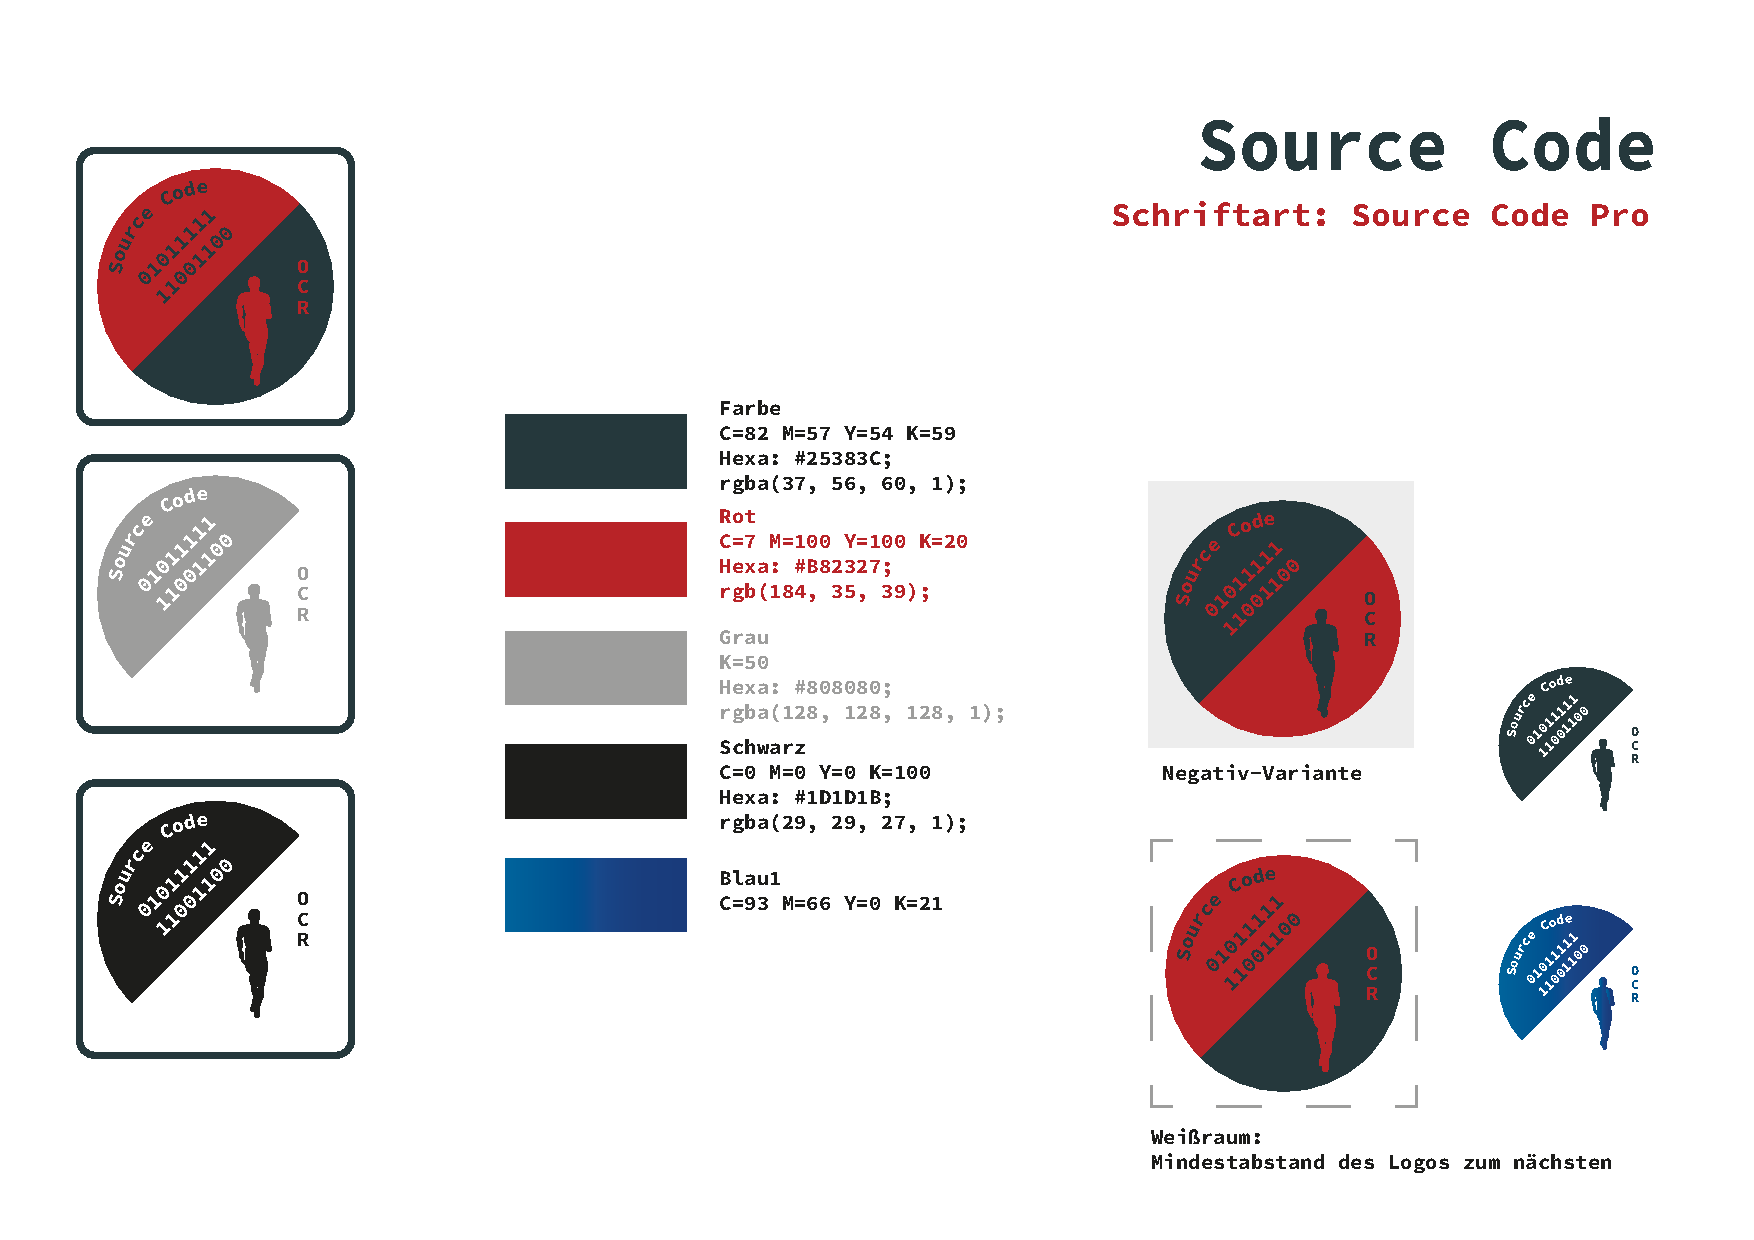
\includepdf[pages=-,landscape]{images/Logo/Logo-Details.pdf}%landscape

	%\input{content/tex/.tex}

	% Bibliographie
    \printbibliography[category=cited]
\end{document}
